\documentclass[]{article}
\usepackage{amsmath, amsfonts}
\usepackage{enumitem}
\usepackage{fancyhdr}
\usepackage{geometry}
\usepackage{cancel}
\usepackage{graphicx}
\usepackage{color}
\usepackage{multirow}
\usepackage{float}
\usepackage{pgfplots}	% To draw charts directly in Latex
\usepackage{marvosym}	% For lightning symbol to denote contradiction

%TikZ package for drawing:
\usepackage{tikz}
%For calculation of coordinates:
\usetikzlibrary{calc}
\usetikzlibrary{positioning}

%opening
\title{Problem Set III \\ \large Microeconomics II}
\author{Nurfatima Jandarova}
\date{\today}
\pagestyle{fancy}

\lhead{Microeconomics II, Problem Set III}
\rhead{Nurfatima Jandarova}
\renewcommand{\headrulewidth}{0.4pt}
\fancyheadoffset{1 cm}

\geometry{a4paper, left=20mm, top=20mm, bottom = 20mm, headheight=20mm}

\sloppy
\definecolor{lightgray}{gray}{0.5}
\setlength{\parindent}{0pt}

\renewcommand{\arraystretch}{1.3}

\begin{document}

\maketitle

\subsection*{Exercise 1}
\begin{enumerate}[label=(\roman*)]
	\item Imposing an assumption of rationality upon players, we can search for the strictly dominated strategies. Denote the probability of player 1 playing pure strategy $X$ by $\sigma_1$:
	\begin{equation}
		\begin{split}
		\pi_1(Y, A) = 0 &< \sigma_1 = \pi_1(\sigma_1, A),\forall\sigma_1\in(0,1]\\ \nonumber
		\pi_1(Y, B) = 3 &< 3 + \sigma_1 = \pi_1(\sigma_1, B),\forall\sigma_1\in(0,1]
		\end{split}
	\end{equation}
	Hence, by definition, strategy $Y$ is a dominated strategy. By imposing the assumption of common rationality, we could perform IESDS. Denote the probability of player 2 playing a pure strategy $A$ by $\sigma_2$:
	\begin{equation}
		\pi_2(X, B) = 1 < 1 + 2\sigma_2 = \pi_2(X, \sigma_2), \forall\sigma_2\in(0, 1]\nonumber
	\end{equation}
	That is, a pure strategy $B$ is strictly dominated in a second iteration of the game. After the second iteration, there is only one strategy profile left, $(X, A)$, and hence the game is dominance-solvable.
	
	\item The new payoff table is
	\begin{table}[h]
		\centering
		\begin{tabular}{c|c|c}
			& A     & B    \\
			\hline
			X & -1, 3 & 2, 1 \\
			\hline
			Y & 0, 2  & 3, 4
		\end{tabular}
	\end{table}
	The result of the modified game change from the one previously, assuming again common knowledge of rationality. Notice that now strategy $X$ of player 1 is now strictly dominated by any mixed strategy with probability of player 1 choosing $X$ as $\hat{\sigma}_1\in(0, 1)$ 
	\begin{equation}
		\begin{split}
		\pi_1(X, A) = -1 &< -\hat{\sigma}_1 = \pi_1(\hat{\sigma}_1, A)\\ \nonumber
		\pi_1(X, B) = 2 &< 3 - \hat{\sigma}_1 = \pi_1(\hat{\sigma}_1, B)
		\end{split}
	\end{equation}
	In a second iteration, strategy $A$ of player 2 gets strictly dominated by any mixed strategy with probability of player 2 playing $A$ as $\hat{\sigma}_2\in [0, 1)$:
	\begin{equation}
		\pi_2(Y, A) = 2 < 4 - 2\hat{\sigma}_2 = \pi_2(Y, \hat{\sigma}_2)\nonumber
	\end{equation}
	So, after the second iteration we are left with one strategy profile, $(Y, B)$.
	
	\item Now, player 1 has two additional actions, $S$ ("subtract") and $N$ ("don't subtract"), to choose from at the beginning of the game. The game could be presented in an extensive form:
	\begin{figure}[h]
		\begin{center}
			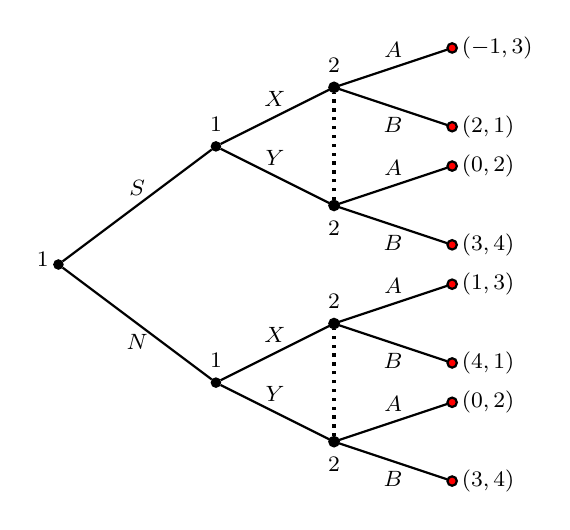
\begin{tikzpicture}
			[
			grow =right,
			font=\footnotesize,
			edge from parent/.style={draw,thick}
			]
			
			% Two node styles: solid and hollow
			\tikzstyle{solid node}=[circle,draw,inner sep=1.2,fill=black];
			\tikzstyle{end node}=[circle,draw,inner sep=1.2,fill=red];
			\tikzstyle{hollow node}=[circle,draw,inner sep=1.2];
			
			% Specify spacing for each level of the tree
			\tikzstyle{level 1}=[level distance=20mm,sibling distance=30mm]
			\tikzstyle{level 2}=[level distance=15mm,sibling distance=15mm]
			\tikzstyle{level 3}=[level distance=15mm,sibling distance=10mm]
			% The Tree
			\node(0)[solid node]{}
			% Don't subtract
			child{node[solid node]{}
				child{node[solid node]{}
					child{node[end node]{} edge from parent node[below]{$B$}}
					child{node[end node]{} edge from parent node[above]{$A$}}
					edge from parent node[align=left, above]{$Y$}
				}
				child{node[solid node]{}
					child{node[end node]{} edge from parent node[below]{$B$}}
					child{node[end node]{} edge from parent node[above]{$A$}}
					edge from parent node[align=left, above]{$X$}
				}
				edge from parent node[align=left, below]{$N$}
			}	
			% Subtract
			child{node[solid node]{}
				child{node[solid node]{}
					child{node[end node]{} edge from parent node[below]{$B$}}
					child{node[end node]{} edge from parent node[above]{$A$}}
					edge from parent node[align=left, above]{$Y$}
				}
				child{node[solid node]{}
					child{node[end node]{} edge from parent node[below]{$B$}}
					child{node[end node]{} edge from parent node[above]{$A$}}
					edge from parent node[align=left, above]{$X$}
				}
				edge from parent node[align=left, above]{$S$}
			}
			;
			% Information sets
			\draw[dotted,very thick](0-1-1)to(0-1-2);
			\draw[dotted,very thick](0-2-1)to(0-2-2);
			
			% Players
			% player 1, turn 1
			\node[left,yshift=2]at(0){1};
			% player 2, turn 2
			\foreach \x in {1, 2} \node[above,yshift=2]at(0-\x){$1$};
			% player 2
			\foreach \x in {1, 2} \node[below,yshift=-2]at(0-\x-1){$2$};
			\foreach \x in {1, 2} \node[above,yshift=2]at(0-\x-2){$2$};
			
			% Specifying payoffs
			% Don't subtract
			\node[right]at(0-1-1-1){$(3, 4)$};
			\node[right]at(0-1-1-2){$(0, 2)$};
			\node[right]at(0-1-2-1){$(4, 1)$};
			\node[right]at(0-1-2-2){$(1, 3)$};
			% Subtract
			\node[right]at(0-2-1-1){$(3, 4)$};
			\node[right]at(0-2-1-2){$(0, 2)$};
			\node[right]at(0-2-2-1){$(2, 1)$};
			\node[right]at(0-2-2-2){$(-1, 3)$};
			\end{tikzpicture}
		\end{center}
	\end{figure}
	The same game could also be presented in strategic form. We have two players: $N = \{1, 2\}$. Their strategy spaces are:
	\begin{equation}
		\begin{split}
		S_1& = \{S, N\}\times\{X, Y\}^2\\\nonumber
		S_2& = \{A, B\}^2
		\end{split}
	\end{equation}
	and their payoff functions are:
	\begin{equation}
	\begin{split}
		&\pi_1: S_1\times S_2 \longrightarrow \{-1, 0, 1, 2, 3, 4\}\\\nonumber
		&\pi_2: S_2\times S_1 \longrightarrow \{1, 2, 3, 4\}
	\end{split}
	\end{equation}
	represented in the table below:
	\begin{table}[h]
		\centering
		\begin{tabular}{c|c|c|c|c}
						& (A, A) 	& (A, B) 	& (B, A) & (B, B) \\
			\hline
			(S, X, X) 	& (-1, 3*) 	& (-1, 3*) 	& (2, 1) & (2, 1) \\
			(S, X, Y) 	& (-1, 3*) 	& (-1, 3*) 	& (2, 1) & (2, 1) \\
			(S, Y, X) 	& (0, 2) 	& (0, 2) 	& (3*, 4*)& (3, 4*) \\
			(S, Y, Y) 	& (0, 2) 	& (0, 2) 	& (3*, 4*)& (3, 4*) \\
			(N, X, X)	& (1*, 3*) 	& (4*, 1) 	& (1, 3*) & (4*, 1) \\
			(N, X, Y) 	& (0, 2)	& (3, 4*) 	& (0, 2) & (3, 4*) \\
			(N, Y, X) 	& (1*, 3*) 	& (4*, 1) 	& (1, 3*) & (4*, 1) \\
			(N, Y, Y) 	& (0, 2)	& (3, 4*) 	& (0, 2) & (3, 4*)
		\end{tabular}
	\end{table}
	To find Nash equilibria in pure strategies we need to find intersection of best responses of players to pure strategies of each other (in the table, I put stars against respective payoffs of players). 
	\begin{equation}
		\begin{split}
		\rho_1(A, A) = \{(N, X, X), (N, Y, X)\} \qquad & \qquad \rho_1(A, B) = \{(N, X, X), (N, Y, X)\} \\ \nonumber
		\rho_1(B, A) = \{(S, Y, X), (S, Y, Y)\} \qquad & \qquad \rho_1(B, B) = \{(N, X, X), (N, Y, X)\} \\
		\rho_2(S, X, X) = \{(A, A), (A, B)\} \qquad & \qquad \rho_2(S, X, Y) = \{(A, A), (A, B)\} \\
		\rho_2(S, Y, X) = \{(B, A), (B, B)\} \qquad & \qquad \rho_2(S, Y, Y) = \{(B, A), (B, B)\} \\
		\rho_2(N, X, X) = \{(A, A), (B, A)\} \qquad & \qquad \rho_2(N, X, Y) = \{(A, B), (B, B)\} \\
		\rho_2(N, Y, X) = \{(A, A), (B, A)\} \qquad & \qquad \rho_2(N, Y, Y) = \{(A, B), (B, B)\}
		\end{split}
	\end{equation}
	So, the set of Nash equilibria in pure strategies is $\{(N, X, X), (A, A)\}, \{(N, Y, X), (A, A)\}$, $\{(S, Y, X), (B, A)\}, \{(S, Y, Y), (B, A)\}$, where the players' best response correspondences intersect.
\end{enumerate}

\subsection*{Exercise 2}
In the first round we can say that strategy $C$ of player 1 is strictly dominated by a mixed strategy $\sigma_1 = (\frac{2}{3}, \frac{1}{3}, 0)$:
\begin{equation}
	\begin{split}
		\pi_1(\sigma_1, R) = 2 + \frac{4}{3}& > 1 = \pi_1(C, R) \\ \nonumber
		\pi_1(\sigma_1, S) = \frac{4}{3}& > 1 = \pi_1(C, S) \\
		\pi_1(\sigma_1, T) = \frac{2}{3} + \frac{2}{3}& > 0 = \pi_1(C, T)
	\end{split}
\end{equation}
In the second round, strategy $T$ of player 2 is strictly dominated by a mixed strategy $\sigma_2 = (\frac{1}{4}, \frac{3}{4}, 0)$:
\begin{equation}
	\begin{split}
		\pi_2(A, \sigma_2) = \frac{3}{2}& > 1 = \pi_2(A, T) \\ \nonumber
		\pi_2(B, \sigma_2) = 1 + \frac{9}{4}& > 2 = \pi_2(B, T)
	\end{split}
\end{equation}
After the second round, there are no strictly dominated strategies. Say, $p\in(0, 1)$ is the probability of player 1 playing $A$ and $q\in(0, 1)$ is the probability of player 2 playing $R$. Then,
\begin{equation}
	\begin{split}
		\pi_1(A, R) = 3 < \pi_1(p, R) &= 3p + 4(1-p) < 4 = \pi_1(B, R) \\ \nonumber
		\pi_1(A, S) = 2 > \pi_1(p, S) &= 2p \qquad\qquad > 0 = \pi_1(B, S) \\
		\pi_2(A, R) = 0 < \pi_2(A, q) &= 2(1-q) \qquad < 2 = \pi_2(A, S) \\
		\pi_2(B, R) = 4 > \pi_2(B, q) &= 4q + 3(1-q) > 3 = \pi_1(B, S)
	\end{split}
\end{equation}
Hence, the following games survives IESDS:
	\begin{table}[h]
	\centering
	\begin{tabular}{c|c|c}
			& R 		& S \\
		\hline
		A 	& (3, 0) 	& (2, 2) \\
		B 	& (4, 4) 	& (0, 3)
	\end{tabular}
\end{table}

Recall that Nash equilibria survive IESDS. Hence, we could restrict our search of NE to the game in the above table. Again, assuming $p$ is the probability of player 1 playing $A$ and $q$ is the probability of player 2 playing $R$, the corresponding payoffs of two players are:
\begin{equation}
	\begin{split}
		\pi_1(p, q)& = q(3p + 4(1-p)) + (1-q)(2p) = 4q - pq + 2p - 2pq = 4q + 2p - 3pq\\ \nonumber
		\pi_2(p, q)& = p(2(1-q)) + (1-p)(4q + 3(1-q)) = 2p - 2pq + q - pq + 3 - 3p = 3 - p + q - 3pq
	\end{split}
\end{equation}
the best response correspondences could be found as:
\begin{equation}
	\begin{split}
		\rho_1(q) = \arg\max\limits_{p}4q + 2p - 3pq = &\begin{cases}
		1 &\text{ for }q < \frac{2}{3} \\
		[0, 1] &\text{ for }q = \frac{2}{3} \\
		0 &\text{ for }q > \frac{2}{3}
		\end{cases}\\ \nonumber
		\rho_2(p) = \arg\max\limits_{q}3 - p + q - 3pq = &\begin{cases}
		1 &\text{ for }p < \frac{1}{3} \\
		[0, 1] &\text{ for }p = \frac{1}{3} \\
		0 &\text{ for }p > \frac{1}{3}
		\end{cases}\\		
	\end{split}
\end{equation}

Thus, there are three Nash equilibria: two in pure strategies $(A, S)$ and $(B, R)$ and one in mixed strategies $(1/3, 2/3)$.
\\
\begin{figure}[h]
	\centering
	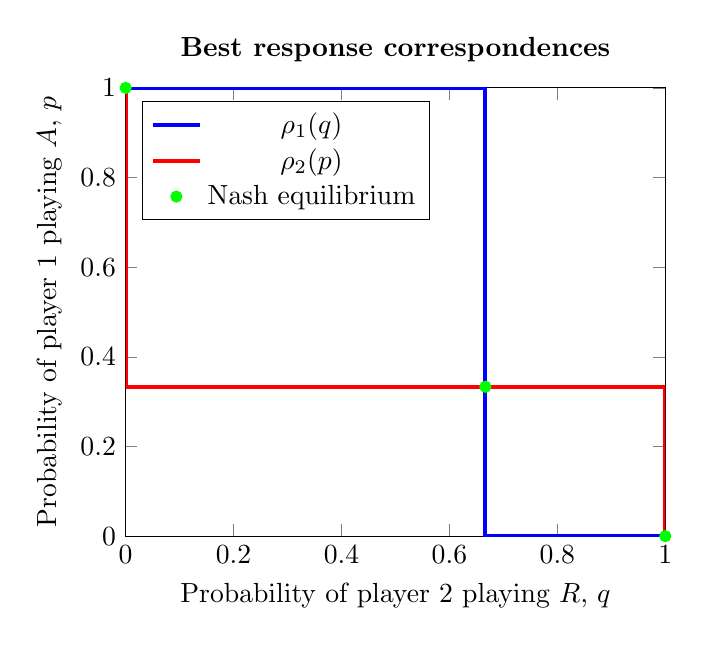
\begin{tikzpicture}
	\begin{axis}[
	title={\textbf{Best response correspondences}},
	xlabel={Probability of player 2 playing $R$, $q$},
	ylabel={Probability of player 1 playing $A$, $p$},
	xmin=0, xmax=1,
	ymin=0, ymax=1,
	legend pos=north west,
	ymajorgrids=false,
	]
	
	% Best response correspondence of player 1
	\addplot [color = blue, line width = 1.5pt]
	coordinates {(0,1)(2/3,1)(2/3,0)(2/3,1)(2/3,0)(1,0)};
	
	% Best response correspondence of player 2
	\addplot[color=red, line width = 1.5pt]
	coordinates {(1,0)(1,1/3)(0,1/3)(1,1/3)(0,1/3)(0,1)};
	
	% Nash equilibria
	\addplot[only marks, color=green, mark = *]
	coordinates {(0,1)(2/3,1/3)(1,0)};
	\legend{$\rho_1(q)$, $\rho_2(p)$, Nash equilibrium}
	\end{axis}
	\end{tikzpicture}
\end{figure}

\subsection*{Exercise 3}

Denote the probability of player 1 playing $T$ as $p_T\in[0, 1]$, $M$ - as $p_M\in[0, 1]$, and $D$ - as $1 - p_T - p_M\in[0, 1]$; and similarly, probability of player 2 playing $L$ - as $q_L\in[0, 1]$, $C$ - as $q_C\in[0, 1]$, and $R$ - as $1 - q_L - q_C\in[0, 1]$. Then, the mixed strategies of two players are $\sigma_1 = (p_T, p_M, 1 - p_T - p_M)$ and $\sigma_2 = (q_L, q_C, 1 - q_L - q_C)$. %Notice that here I also allow for pure strategies described by mixed strategy profiles where one of the probabilities takes value 1.

For Nash equilibrium in mixed strategies to be sustainable we need first to ensure that players get same payoff irrespective of the choice of the pure strategy and that there is no profitable deviation. Hence, need to solve following systems of linear equations:

\begin{equation}
	\begin{split}
		&\begin{cases}
			&q_L + 5q_C = 5q_L + q_C \\
			&q_L + 5q_C = 6(1 - q_L - q_C)
		\end{cases} \Rightarrow \begin{cases}
		&4q_C = 4q_L \\
		&7q_L + 11q_C = 6
		\end{cases} \Rightarrow \begin{cases}
		&q_C = \frac{1}{3} \\
		&q_L = \frac{1}{3}		
		\end{cases} \\ \nonumber
		&\begin{cases}
		&3p_T + p_M + 2(1 - p_T - p_M) = 4(1 - p_T - p_M) \\
		&4(1 - p_T - p_M) = 2p_T + 6p_M
		\end{cases} \Rightarrow \begin{cases}
		&5p_T + 3p_M = 2 \\
		&6p_T + 10p_M = 4
		\end{cases} \Rightarrow \begin{cases}
		&p_T = \frac{2 - 3p_M}{5} \\
		&32p_M = 8
		\end{cases} \Rightarrow \begin{cases}
		&p_T = \frac{1}{4} \\
		&p_M = \frac{1}{4}
		\end{cases}
	\end{split}
\end{equation}
Hence, the mixed strategies of the two players is described by $\sigma_1 = (\frac{1}{4}, \frac{1}{4}, \frac{1}{2})$ and $\sigma_2 = (\frac{1}{3}, \frac{1}{3}, \frac{1}{3})$ that yield the expected payoffs $\mathbb{E}(\pi_1(\sigma_1, \sigma_2)) = \frac{1}{3}\begin{pmatrix}\frac{1}{4} + \frac{5}{4} + \frac{5}{4} + \frac{1}{4} + \frac{6}{2}\end{pmatrix} = 2$ and $\mathbb{E}(\pi_2(\sigma_1, \sigma_2)) = \frac{1}{4}\frac{3+2+1+6}{3} + \frac{1}{2}\frac{2 + 4}{3} = 2$.

Now, suppose that player 1 considers a deviation to $\hat{\sigma}_1 = (\frac{1-\epsilon}{4}, \frac{1}{4}, \frac{1+\frac{\epsilon}{2}}{2}), \forall\mid\epsilon\mid<1$. Then, the expected payoff is $\mathbb{E}(\pi_1(\hat{\sigma}_1, \sigma_2)) = \frac{1}{3}\begin{pmatrix}\frac{1 - \epsilon}{4} + \frac{5}{4} + \frac{5(1 - \epsilon)}{4} + \frac{1}{4} + \frac{6(1 + \frac{\epsilon}{2})}{2}\end{pmatrix} = \frac{1}{3}\begin{pmatrix}\frac{6 - 6\epsilon + 12 + 6\epsilon}{4} + \frac{6}{4}\end{pmatrix} = 2$. Thus, there is no profitable deviation for player 1. 

Similarly, if player 2 considers deviating to $\hat{\sigma}_2 = (\frac{1+\epsilon}{3}, \frac{1}{3}, \frac{1-\epsilon}{3}), \forall\mid\epsilon\mid<1$. Then, $\mathbb{E}(\pi_2(\sigma_1, \hat{\sigma}_2)) = \frac{1}{4}\begin{pmatrix}\frac{3(1 + \epsilon)}{3} + \frac{2(1 - \epsilon)}{3} + \frac{1 + \epsilon}{3} + \frac{6(1 - \epsilon)}{3}\end{pmatrix} + \frac{1}{2}\begin{pmatrix}\frac{2(1 + \epsilon)}{3} + \frac{4}{3}\end{pmatrix} = 2$. Again, no profitable deviation for player 2.

Thus, $(\sigma_1, \sigma_2)$ is a Nash equilibrium.

\subsection*{Exercise 5}
\begin{enumerate}[label=(\roman*)]
	\item Denote the probability of player 1 choosing $A$ as $p\in[0 ,1]$ and the probability of player 2 choosing $C$ as $q\in[0, 1]$. Then, the payoffs of the two players are:
	\begin{equation}
	\pi_1(p, q) = \begin{bmatrix}p & 1 - p\end{bmatrix}\begin{bmatrix}3 & -1 \\ -2 & 1\end{bmatrix}\begin{bmatrix}q \\ 1 - q\end{bmatrix} = -\pi_2(p, q) \nonumber
	\end{equation}
	
	Then, 
	\begin{equation}
		\begin{split}
		\rho_1(q) = \arg\max\limits_{p}1 - 2p - 3q + 7pq = &\begin{cases}
		1&\text{ for }q > \frac{2}{7} \\
		[0, 1]&\text{ for }q = \frac{2}{7} \\
		0&\text{ for }q < \frac{2}{7}
		\end{cases}\\ \nonumber
		\rho_2(p) = \arg\max\limits_{q} -1 + 2p + 3q - 7pq = &\begin{cases}
		1&\text{ for }p < \frac{3}{7} \\
		[0, 1]&\text{ for }p = \frac{3}{7} \\
		0&\text{ for }p > \frac{3}{7}
		\end{cases}
		\end{split}
	\end{equation}
	\begin{figure}[h]
		\centering
		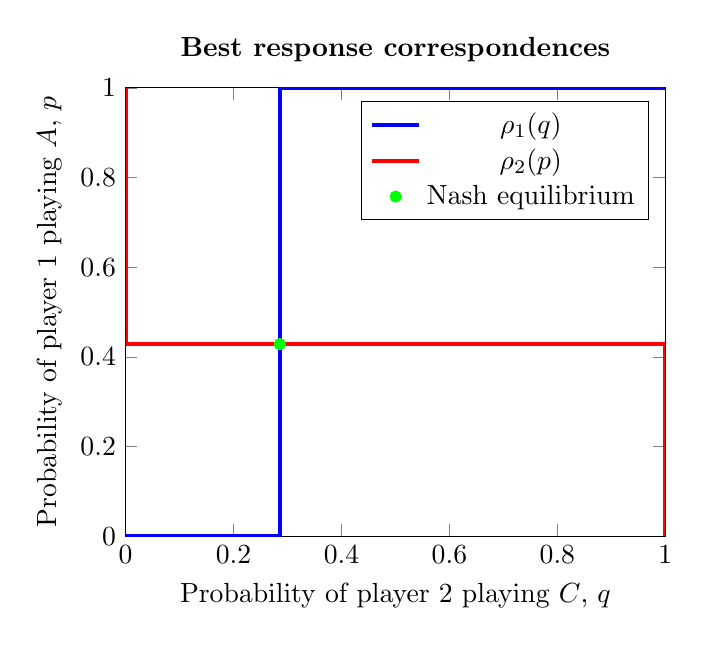
\begin{tikzpicture}
		\begin{axis}[
		title={\textbf{Best response correspondences}},
		xlabel={Probability of player 2 playing $C$, $q$},
		ylabel={Probability of player 1 playing $A$, $p$},
		xmin=0, xmax=1,
		ymin=0, ymax=1,
		legend pos=north east,
		ymajorgrids=false,
		]
		% Best response correspondence of player 1
		\addplot [color = blue, line width = 1.5pt]
		coordinates {(0,0)(2/7,0)(2/7,0)(2/7,1)(2/7,1)(1,1)};
		
		% Best response correspondence of player 2
		\addplot[color=red, line width = 1.5pt]
		coordinates {(1,0)(1,3/7)(0,3/7)(1,3/7)(0,3/7)(0,1)};
		
		% Nash equilibria
		\addplot[only marks, color=green, mark = *]
		coordinates {(2/7,3/7)};
		\legend{$\rho_1(q)$, $\rho_2(p)$, Nash equilibrium}
		\end{axis}
		\end{tikzpicture}
	\end{figure}
	
	Hence, the Nash equilibrium is a mixed strategy $(p, q) = (\frac{3}{7}, \frac{2}{7})$ and the expected payoffs are $\pi_1(\frac{3}{7}, \frac{2}{7}) = \frac{1}{7} = -\pi_2(\frac{3}{7}, \frac{2}{7})$.
	
	\item Recall that $v_1 = \max\limits_{p}\min\limits_{q}1 - 2p - 3q + 7pq$. Let's consider the inner minimization problem
	\begin{equation}
		\begin{split}
		\arg\min\limits_{q}1 - 2p - 3q + 7pq = \begin{cases}
		1&\text{for }p < \frac{3}{7}\\
		[0, 1]&\text{for }p = \frac{3}{7}\\
		0&\text{for }p > \frac{3}{7}
		\end{cases} \Rightarrow \min\limits_{q}1 - 2p - 3q + 7pq = \begin{cases}
		5p - 2&\text{for }p < \frac{3}{7}\\
		1 - 2p - 3q + 7pq&\text{for }p = \frac{3}{7}\\
		1 - 2p&\text{for }p > \frac{3}{7}
		\end{cases}\nonumber
		\end{split}
	\end{equation}
	
	Suppose, player 2 believes $p < \frac{3}{7}$ and adopts $q = 1$. Then, player 1's objective is to $\max\limits_{p}5p - 2$, i.e., set $p = 1\Rightarrow$ \Lightning. Similarly, suppose player 2  believes $p > \frac{3}{7}$ and sets $q = 0$. Then player 1 wants to $\max\limits_{p}1 - 2p$, which implies that he/she wants to set $p = 0\Rightarrow$ \Lightning. If player 2 believes that $p = \frac{3}{7}$, then player 2 is indifferent between any probability in [0, 1], which means that player 1's problem is characterized by $\rho_1(q)$ in the first part of this exercise. Following similar reasoning, if player 2 sets $q > \frac{2}{7}$, player 1 adopts $p = 1$, which again leads to contradiction; if player 2 sets $q < \frac{2}{7}$, player 1 chooses $p = 0 \Rightarrow$ \Lightning. Hence, the only stable solution is achieved with the strategy $(p, q) = (\frac{3}{7}, \frac{2}{7})$ and $v_1 = \frac{1}{7}$. As is evident from the reasoning above, to achieve this solution we used the notion of common knowledge of rationality.
	
	Repeating the same procedure for the second player we get:
	\begin{equation}
		\begin{split}
		v_2 &= \min\limits_{q}\max\limits_{p}1 - 2p - 3q + 7pq \\ \nonumber
		\arg\max\limits_{p}1 - 2p - 3q + 7pq = \begin{cases}
		1&\text{for }q > \frac{2}{7} \\
		[0, 1]&\text{for }q = \frac{2}{7} \\
		0&\text{for }q < \frac{2}{7}
		\end{cases} &\Rightarrow \max\limits_{p}1 - 2p - 3q + 7pq = \begin{cases}
		4q - 1&\text{for }q > \frac{2}{7} \\
		1 - 2p - 3q + 7pq&\text{for }q = \frac{2}{7} \\
		1 - 3q&\text{for }q < \frac{2}{7}
		\end{cases}
		\end{split}
	\end{equation}
	Again, if player 1 believes that $q < \frac{2}{7}$, then player 2's objective is to $\min\limits_{q}1 - 3q$, i.e., set $q = 1\Rightarrow$ \Lightning. If player 1 believes that $q > \frac{2}{7}$, then player 2 wants to $\min\limits_{q}4q - 1$ and chooses $q = 0\Rightarrow$ \Lightning. And again, the only stable solution is achieved when $(p, q) = (\frac{3}{7}, \frac{2}{7})$, hence, $v_2 = \frac{1}{7}$.
\end{enumerate}

\subsection*{Exercise 4}

We have a set of players $N = \{1, 2\}$, strategy spaces $S_1 = \{A, B, C, D\}$ and $S_2 = \{A, B, C, D\}$ and payoffs $\pi_1(s_{1k}, s_{2l}) = a_{kl} = -\pi_2(s_{1k}, s_{2l})$, where $s_{ik}$ is the $k^\text{th}$ strategy of player $i$. Hence, the game in the strategic form could be described as $G = \{N, S_1\times S_2, \{\pi_1, \pi_2\}\}$. Since this is the zero-sum game payoffs of both players could be specified using matrix $A$ defined as follows:
\begin{equation}
A = \begin{pmatrix}
4 & 2 & 0 & 4 \\
3 & 3 & 3 & 3 \\
0 & 0 & 4 & 4 \\
1 & 1 & 0 & 1
\end{pmatrix} \nonumber
\end{equation}

This allows us to write the payoffs for any mixed strategies as:
\begin{equation}
\pi_1(\sigma_1, \sigma_2) = \sigma_1A\sigma_2 = -\pi_2(\sigma_1, \sigma_2), \forall (\sigma_1, \sigma_2) \in \Sigma_1\times\Sigma_2 \nonumber
\end{equation}

\begin{enumerate}[label=(\roman*)]
	\item Recall that $v_1 = \max\limits_{\sigma_1}\min\limits_{\sigma_2}\sigma_1A\sigma_2$. Notice that $\forall (\sigma_1, \sigma_2)\in\Sigma_1\times\Sigma_2, \pi_1(\sigma_1, \sigma_2)$ is convex combination of $\pi_1(\sigma_1, (1, 0, 0, 0)), \pi_1(\sigma_1, (0, 1, 0, 0)), \pi_1(\sigma_1, (0, 0, 1, 0))$, and $\pi_1(\sigma_1, (0, 0, 0, 1))$, i.e., these are worst/best cases. Therefore, the optimization problem of player 1 is $\max\{4\sigma_{11} + 3\sigma_{12} + \sigma_{14}, 2\sigma_{11} + 3\sigma_{12} + \sigma_{14}, 3\sigma_{12} + 4\sigma_{13}, 4\sigma_{11} + 3\sigma_{12} + 4\sigma_{13} + \sigma_{14}\}$, where $\sigma_{ik}$ is the probability assigned to the $k^\text{th}$ strategy of player $i$. Hence, the first player solves following system of linear equations:
	\begin{equation}
		\begin{split}
			\begin{cases}
				&4\sigma_{11} + 3\sigma_{12} + \sigma_{14} = 2\sigma_{11} + 3\sigma_{12} + \sigma_{14} \\
				&3\sigma_{12} + 4\sigma_{13} = 4\sigma_{11} + 3\sigma_{12} + 4\sigma_{13} + \sigma_{14} \\
				&3\sigma_{12} + 4\sigma_{13} = 2\sigma_{11} + 3\sigma_{12} + \sigma_{14} \\
				&\sigma_{11} + \sigma_{12} + \sigma_{13} + \sigma_{14} = 0
			\end{cases} \Rightarrow
			\begin{cases}
				&\sigma_{11} = 0 \\
				&\sigma_{14} = 0 \\
				&\sigma_{13} = 0 \\
				&\sigma_{12} = 1
			\end{cases} \nonumber
		\end{split}
	\end{equation}
	Then, the first player gets the expected payoff of $v_1 = \pi_1((0, 1, 0, 0), \sigma_{2}) = 3\sigma_{21} + 3\sigma_{22} + 3\sigma_{23} + 3\sigma_{24} = 3$. Hence, the maxmin strategy of player 1 is to play $B$ regardless of what the second does and the player 2 is indifferent between any distribution of probabilities over $S_2$.
	
	\item Similar to the previous part of this exercise, $v_2 = \min\limits_{\sigma_2}\max\limits_{\sigma_1}\sigma_1A\sigma_2$, and again payoff of any strategy profile is a linear combination of $\pi_2((1, 0, 0, 0), \sigma_2), \pi_2((0, 1, 0, 0), \sigma_2), \pi_2((0, 0, 1, 0), \sigma_2)$, and $\pi_2((0, 0, 0, 1), \sigma_2)$, i.e., the optimization problem of player 2 is $\min\{4\sigma_{21} + 2\sigma_{22} + 4\sigma_{24}, 3, 4\sigma_{23} + 4\sigma_{24}, \sigma_{21} + \sigma_{22} + \sigma_{24}\}$.
	\begin{equation}
		\begin{cases}
			&4\sigma_{21} + 2\sigma_{22} + 4\sigma_{24} = 3 \\
			&4\sigma_{23} + 4\sigma_{24} = 3 \\
			&\sigma_{21} + \sigma_{22} + \sigma_{24} = 3 \Longrightarrow \emptyset\\
			&\sigma_{21} + \sigma_{22} + \sigma_{23} + \sigma_{24} = 1
		\end{cases}
	\end{equation}
	Hence, there is no solution to minmax problem of the second player and $v_2=\emptyset$.
	
	\item There is a Nash equilibrium in pure strategies, $(B, B)$, where player's best responses to pure strategies of each other intersect. 
	\begin{figure}[h]
		\centering
		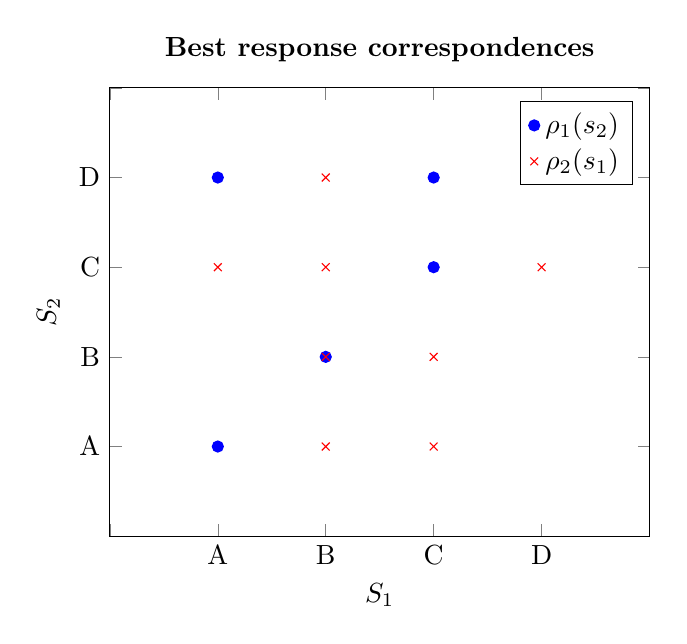
\begin{tikzpicture}
		\begin{axis}[
		title={\textbf{Best response correspondences}},
		xlabel={$S_1$},
		xticklabels={, , A, B, C, D},
		ylabel={$S_2$},
		yticklabels={, , A, B, C, D},
		xmin=0, xmax=5,
		ymin=0, ymax=5,
		legend pos=north east,
		ymajorgrids=false,
		]
		
		% Best response correspondence of player 1
		\addplot[only marks, color = blue, mark = *]
		coordinates {(1,1)(2,2)(3,3)(1,4)(3,4)};
		
		% Best response correspondence of player 2
		\addplot[only marks, color=red, mark = x]
		coordinates {(1,3)(2,1)(2,2)(2,3)(2,4)(3,1)(3,2)(4,3)};
		
		\legend{$\rho_1(s_2)$, $\rho_2(s_1)$}
		\end{axis}
		\end{tikzpicture}
	\end{figure}

	Using the results above we can say that there is no mixed strategy for player 1 as we have seen there doesn't exist $\sigma_2$ such that player 1 is indifferent between his/her strategies. 
\end{enumerate}

\end{document}
